\documentclass[12pt,a4paper]{article}

% ─── Packages ────────────────────────────────────────────────────────────────
\usepackage{amsmath, amssymb, amsthm}
\usepackage{geometry}
\usepackage{hyperref}
\usepackage{tikz}
\usepackage{pgfplots}
\pgfplotsset{compat=1.18}
\usetikzlibrary{arrows.meta, calc, positioning, shapes.geometric,
	decorations.pathreplacing, backgrounds, fit, matrix}
\usepackage{xcolor}
\usepackage{tcolorbox}
\tcbuselibrary{theorems, skins, breakable}
\usepackage{booktabs}
\usepackage{array}
\usepackage{enumitem}
\usepackage{mathrsfs}
\usepackage{fancyhdr}
\usepackage{titlesec}
\usepackage{microtype}
\usepackage{setspace}

% ─── Page Geometry ────────────────────────────────────────────────────────────
\geometry{margin=2.5cm, top=3cm, bottom=3cm}
\setlength{\headheight}{14pt}
\setstretch{1.15}

% ─── Colours ──────────────────────────────────────────────────────────────────
\definecolor{axiomblue}{RGB}{30, 80, 160}
\definecolor{defgreen}{RGB}{20, 130, 80}
\definecolor{thmred}{RGB}{160, 30, 40}
\definecolor{notegray}{RGB}{90, 90, 90}
\definecolor{shadeblue}{RGB}{230, 240, 255}
\definecolor{shadegreen}{RGB}{225, 248, 235}
\definecolor{shadered}{RGB}{255, 235, 235}
\definecolor{shadeyellow}{RGB}{255, 252, 220}
\definecolor{purpleshade}{RGB}{240, 230, 255}
\definecolor{purpledark}{RGB}{100, 30, 160}
\definecolor{orangeshade}{RGB}{255, 243, 225}
\definecolor{orangedark}{RGB}{180, 90, 0}

% ─── Header / Footer ─────────────────────────────────────────────────────────
\pagestyle{fancy}
\fancyhf{}
\fancyhead[L]{\small\textit{Linear Algebra}}
\fancyhead[R]{\small\textit{Linear Independence, Basis \& Dimension}}
\fancyfoot[C]{\thepage}
\renewcommand{\headrulewidth}{0.4pt}

% ─── Section Formatting ───────────────────────────────────────────────────────
\titleformat{\section}{\large\bfseries\color{axiomblue}}{\thesection}{1em}{}[\titlerule]
\titleformat{\subsection}{\normalsize\bfseries\color{defgreen}}{\thesubsection}{1em}{}
\titleformat{\subsubsection}{\normalsize\bfseries\color{notegray}}{\thesubsubsection}{1em}{}

% ─── Theorem Environments ─────────────────────────────────────────────────────
\tcbset{
	defstyle/.style={
		enhanced, colback=shadegreen, colframe=defgreen,
		fonttitle=\bfseries, breakable
	},
	thmstyle/.style={
		enhanced, colback=shadered, colframe=thmred,
		fonttitle=\bfseries, breakable
	},
	axiomstyle/.style={
		enhanced, colback=shadeblue, colframe=axiomblue,
		fonttitle=\bfseries, breakable
	},
	notestyle/.style={
		enhanced, colback=shadeyellow, colframe=orange!70!black,
		fonttitle=\bfseries, breakable
	},
	propstyle/.style={
		enhanced, colback=purpleshade, colframe=purpledark,
		fonttitle=\bfseries, breakable
	},
	corstyle/.style={
		enhanced, colback=orangeshade, colframe=orangedark,
		fonttitle=\bfseries, breakable
	}
}

\newtcbtheorem[number within=section]{definition}{Definition}{defstyle}{def}
\newtcbtheorem[number within=section]{theorem}{Theorem}{thmstyle}{thm}
\newtcbtheorem[number within=section]{corollary}{Corollary}{corstyle}{cor}
\newtcbtheorem[number within=section]{proposition}{Proposition}{propstyle}{prop}
\newtcbtheorem[number within=section]{remark}{Remark}{notestyle}{rem}
\newtcbtheorem[number within=section]{example}{Example}{notestyle}{ex}

% ─── Math Operators ───────────────────────────────────────────────────────────
\newcommand{\R}{\mathbb{R}}
\newcommand{\vv}[1]{\mathbf{#1}}
\newcommand{\vzero}{\mathbf{0}}
\newcommand{\norm}[1]{\left\lVert #1 \right\rVert}
\DeclareMathOperator{\Span}{Span}
\DeclareMathOperator{\rank}{rank}
\DeclareMathOperator{\nullity}{nullity}
\renewcommand{\qedsymbol}{$\blacksquare$}

% ══════════════════════════════════════════════════════════════════════════════
\begin{document}
	% ══════════════════════════════════════════════════════════════════════════════
	
	% ─── Title Page ───────────────────────────────────────────────────────────────
	% NOTE: Only pure TikZ inside titlepage – no pgfplots \begin{axis} here.
		\begin{titlepage}
			\centering
			\vspace*{3cm}
			{\Huge\bfseries\color{axiomblue} Linear Algebra}\\[0.8em]
			{\huge\bfseries Linear Independence, Basis \& Dimension}\\[2em]
			\rule{0.6\linewidth}{1.5pt}\\[2em]
			{\large\itshape A Comprehensive Mathematical Treatment}\\[1em]
			{\normalsize Covering linear independence and dependence,\\
				bases of vector spaces, the dimension theorem,\\
				and the Rank--Nullity theorem.}\\[4em]
			% Pure TikZ cover diagram: dependent vs independent vectors
			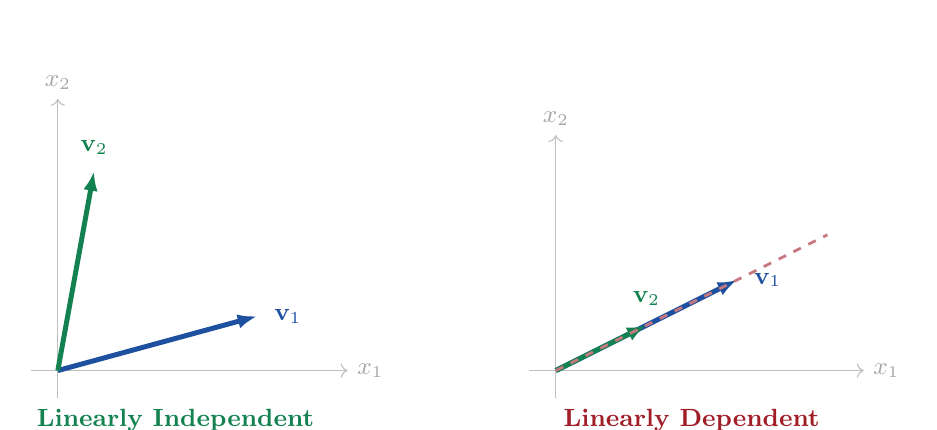
\begin{tikzpicture}[scale=1.15,
				vecA/.style={-{Latex[length=7pt]}, axiomblue, line width=1.8pt},
				vecB/.style={-{Latex[length=7pt]}, defgreen, line width=1.8pt},
				vecC/.style={-{Latex[length=7pt]}, thmred, line width=1.8pt}]
				%--- Left panel: linearly independent ---
				\begin{scope}
					\draw[->, gray!50, thin] (-0.3,0) -- (3.2,0)
					node[right, gray!70, font=\small]{$x_1$};
					\draw[->, gray!50, thin] (0,-0.3) -- (0,3.0)
					node[above, gray!70, font=\small]{$x_2$};
					\draw[vecA] (0,0) -- (2.2,0.6)
					node[right=2pt, font=\small]{$\vv{v}_1$};
					\draw[vecB] (0,0) -- (0.4,2.2)
					node[above=2pt, font=\small]{$\vv{v}_2$};
					\node[font=\small\bfseries\color{defgreen}] at (1.3,-0.55)
					{Linearly Independent};
				\end{scope}
				%--- Right panel: linearly dependent ---
				\begin{scope}[xshift=5.5cm]
					\draw[->, gray!50, thin] (-0.3,0) -- (3.4,0)
					node[right, gray!70, font=\small]{$x_1$};
					\draw[->, gray!50, thin] (0,-0.3) -- (0,2.6)
					node[above, gray!70, font=\small]{$x_2$};
					\draw[vecA] (0,0) -- (2.0,1.0)
					node[right=2pt, font=\small]{$\vv{v}_1$};
					\draw[vecB] (0,0) -- (1.0,0.5)
					node[above=3pt, font=\small]{$\vv{v}_2$};
					% dashed: v1 = 2*v2
					\draw[dashed, thmred!60, line width=1pt]
					(0,0) -- (3.0,1.5);
					\node[font=\small\bfseries\color{thmred}] at (1.5,-0.55)
					{Linearly Dependent};
				\end{scope}
			\end{tikzpicture}\\[2em]
			\vfill
			{\small\color{notegray}\today}
		\end{titlepage}
		
		% ─── Table of Contents ───────────────────────────────────────────────────────
		\tableofcontents
		\newpage
		
		% ══════════════════════════════════════════════════════════════════════════════
		\section{Introduction}
		% ══════════════════════════════════════════════════════════════════════════════
		
		The notions of \textbf{linear independence}, \textbf{basis}, and
		\textbf{dimension} are the cornerstones of linear algebra.  Together they allow
		us to measure, in a precise algebraic sense, the ``size'' of a vector space and
		to identify the most economical sets of vectors that completely describe it.
		
		Building on the theory of vector spaces and subspaces from the previous chapters,
		this chapter answers three fundamental questions:
		
		\begin{itemize}[leftmargin=2em, itemsep=0.4em]
			\item When is a set of vectors \emph{redundant} in the sense that one of them
			can be expressed as a combination of the others?
			\item What is the smallest spanning set for a vector space?
			\item How many vectors are in every such minimal spanning set?
		\end{itemize}
		
		% ══════════════════════════════════════════════════════════════════════════════
		\section{Linear Independence}
		\label{sec:lindep}
		% ══════════════════════════════════════════════════════════════════════════════
		
		\subsection{Definition}
		
		\begin{definition}{Linear Independence and Dependence}{lindef}
			Let $\vv{v}_1, \vv{v}_2, \ldots, \vv{v}_n$ be vectors in a vector space $V$.
			The vectors are said to be \textbf{linearly dependent} if there exist scalars
			$\alpha_1, \alpha_2, \ldots, \alpha_n$, \emph{not all zero}, such that
			\[
			\alpha_1\vv{v}_1 + \alpha_2\vv{v}_2 + \cdots + \alpha_n\vv{v}_n = \vzero.
			\]
			If the \emph{only} solution to the above equation is
			$\alpha_1 = \alpha_2 = \cdots = \alpha_n = 0$, the vectors are said to be
			\textbf{linearly independent}.
		\end{definition}
		
		\begin{remark}{Intuitive Interpretation}{intuitli}
			Linear dependence means that at least one vector in the set is
			\emph{redundant}: it can be written as a linear combination of the others.
			Concretely, if $\alpha_1 \neq 0$ in a non-trivial relation, then
			\[
			\vv{v}_1 = -\frac{\alpha_2}{\alpha_1}\vv{v}_2
			- \cdots
			- \frac{\alpha_n}{\alpha_1}\vv{v}_n.
			\]
			Linear independence, by contrast, means no vector in the set can be expressed
			this way; every vector contributes a genuinely new ``direction''.
		\end{remark}
		
		\subsection{Testing Linear Independence}
		
		\noindent
		To test whether $\vv{v}_1, \ldots, \vv{v}_n \in \R^m$ are linearly independent,
		form the homogeneous system with coefficient matrix
		$A = [\,\vv{v}_1 \;\vv{v}_2 \;\cdots\; \vv{v}_n\,]$ and solve $A\vv{c} = \vzero$:
		
		\begin{center}
			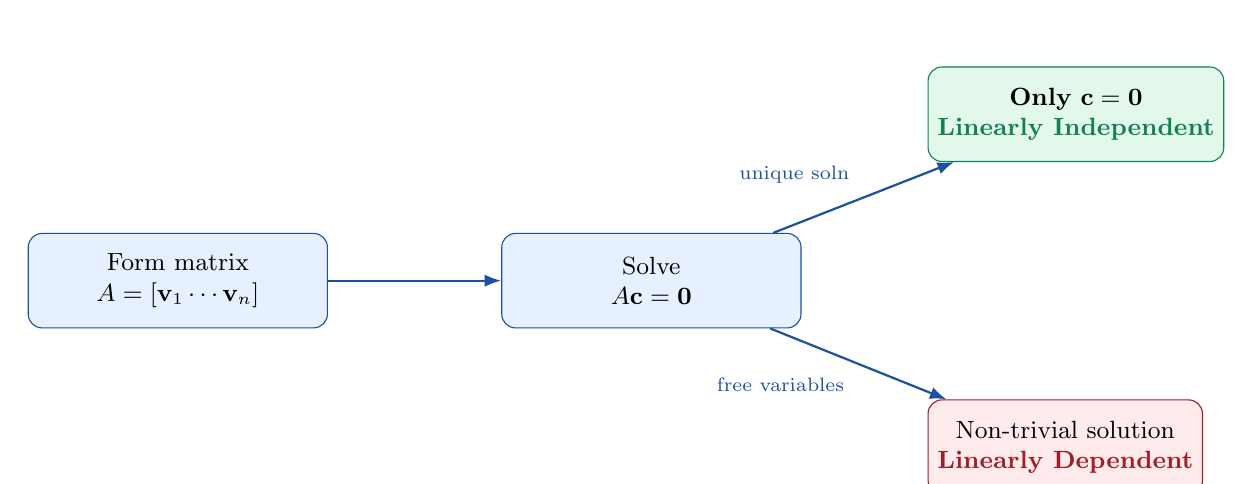
\begin{tikzpicture}[
				node distance=0.5cm and 2.2cm,
				% NOTE: style name 'testbox' avoids conflict with TikZ built-in 'step' key
				testbox/.style={draw=axiomblue, fill=shadeblue, rounded corners=5pt,
					minimum width=3.8cm, minimum height=1.2cm,
					align=center, font=\small},
				resultbox/.style={rounded corners=5pt, minimum width=3.4cm,
					minimum height=1.2cm, align=center, font=\small},
				arr/.style={-{Latex[length=6pt]}, thick, axiomblue}
				]
				\node[testbox] (form)
				{Form matrix\\$A=[\vv{v}_1\cdots\vv{v}_n]$};
				\node[testbox, right=of form] (solve)
				{Solve\\$A\vv{c}=\vzero$};
				\node[resultbox, draw=defgreen, fill=shadegreen,
				above right=0.9cm and 1.6cm of solve] (indep)
				{\textbf{Only} $\vv{c}=\vzero$\\\textcolor{defgreen}{\bfseries Linearly Independent}};
				\node[resultbox, draw=thmred, fill=shadered,
				below right=0.9cm and 1.6cm of solve] (dep)
				{Non-trivial solution\\\textcolor{thmred}{\bfseries Linearly Dependent}};
				\draw[arr] (form) -- (solve);
				\draw[arr] (solve) -- (indep)
				node[midway, above left=2pt, font=\scriptsize]{unique soln};
				\draw[arr] (solve) -- (dep)
				node[midway, below left=2pt, font=\scriptsize]{free variables};
			\end{tikzpicture}
		\end{center}
		
		\subsection{Examples in \texorpdfstring{$\R^n$}{Rn}}
		
		\begin{example}{Linearly independent vectors in $\R^3$}{liindep}
			Determine whether
			$\vv{v}_1 = (1,\,0,\,2)^T$,
			$\vv{v}_2 = (2,\,1,\,0)^T$,
			$\vv{v}_3 = (0,\,1,\,-4)^T$
			are linearly independent.
			
			Form $A = [\vv{v}_1\;\vv{v}_2\;\vv{v}_3]$ and row-reduce:
			\[
			\begin{pmatrix}
				1 & 2 &  0 \\
				0 & 1 &  1 \\
				2 & 0 & -4
			\end{pmatrix}
			\xrightarrow{R_3 - 2R_1}
			\begin{pmatrix}
				1 & 2 &  0 \\
				0 & 1 &  1 \\
				0 &-4 & -4
			\end{pmatrix}
			\xrightarrow{R_3 + 4R_2}
			\begin{pmatrix}
				1 & 2 & 0 \\
				0 & 1 & 1 \\
				0 & 0 & 0
			\end{pmatrix}.
			\]
			The system $A\vv{c} = \vzero$ has a free variable ($c_3 = t$), giving the
			non-trivial solution $\vv{c} = t(-2,\,-1,\,1)^T$.  Therefore the vectors are
			\textbf{linearly dependent}.  Indeed:
			\[
			-2\vv{v}_1 - \vv{v}_2 + \vv{v}_3
			= \begin{pmatrix}-2\\0\\-4\end{pmatrix}
			+ \begin{pmatrix}-2\\-1\\0\end{pmatrix}
			+ \begin{pmatrix}0\\1\\-4\end{pmatrix}
			= \begin{pmatrix}-4\\0\\-8\end{pmatrix}
			\neq \vzero.
			\]
			(Scaling by $-\tfrac{1}{2}$: $\vv{v}_1 + \tfrac{1}{2}\vv{v}_2 -
			\tfrac{1}{2}\vv{v}_3 = \vzero$, confirming dependence.)
		\end{example}
		
		\begin{example}{Linearly independent vectors in $\R^3$}{liindep2}
			Determine whether
			$\vv{u}_1 = (1,\,0,\,0)^T$,
			$\vv{u}_2 = (0,\,1,\,0)^T$,
			$\vv{u}_3 = (0,\,0,\,1)^T$
			are linearly independent.
			
			The system $A\vv{c} = \vzero$ with
			$A = [\vv{u}_1\;\vv{u}_2\;\vv{u}_3] = I_3$ reduces immediately:
			\[
			I_3\vv{c} = \vzero \;\Longrightarrow\; \vv{c} = \vzero.
			\]
			The only solution is the trivial one, so the vectors are
			\textbf{linearly independent}.
		\end{example}
		
		\subsection{Geometric Interpretation}
		
		\noindent
		In $\R^2$ and $\R^3$, linear (in)dependence has a clear geometric meaning:
		
		\begin{center}
			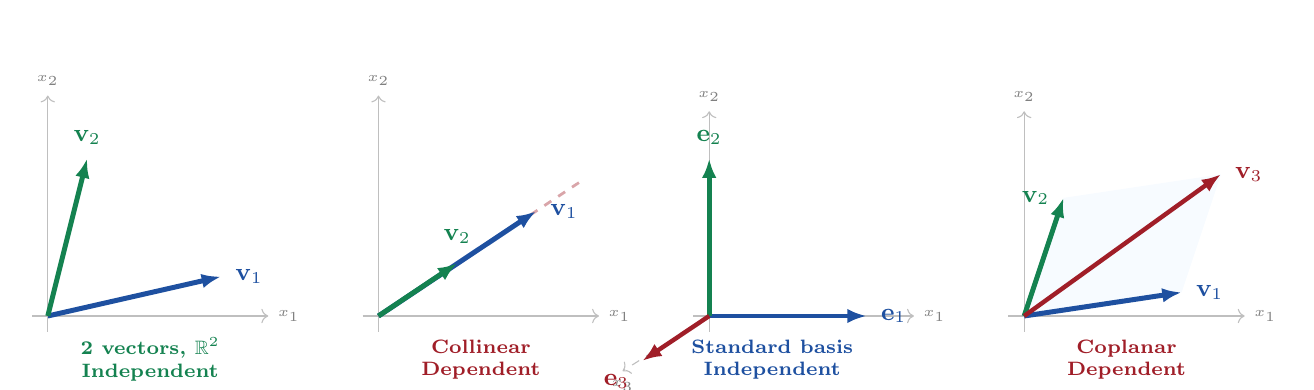
\begin{tikzpicture}[scale=1.0,
				va/.style={-{Latex[length=7pt]}, axiomblue, line width=1.8pt},
				vb/.style={-{Latex[length=7pt]}, defgreen, line width=1.8pt},
				vc/.style={-{Latex[length=7pt]}, thmred, line width=1.6pt}]
				
				%--- Panel 1: 2 independent in R^2 ---
				\begin{scope}
					\draw[->,gray!50,thin](-0.2,0)--(2.8,0)node[right,gray,font=\tiny]{$x_1$};
					\draw[->,gray!50,thin](0,-0.2)--(0,2.8)node[above,gray,font=\tiny]{$x_2$};
					\draw[va](0,0)--(2.2,0.5)node[right=1pt,font=\small]{$\vv{v}_1$};
					\draw[vb](0,0)--(0.5,2.0)node[above=1pt,font=\small]{$\vv{v}_2$};
					\node[font=\scriptsize\bfseries\color{defgreen}, align=center] at (1.3,-0.55)
					{2 vectors, $\R^2$\\Independent};
				\end{scope}
				
				%--- Panel 2: 2 dependent in R^2 (collinear) ---
				\begin{scope}[xshift=4.2cm]
					\draw[->,gray!50,thin](-0.2,0)--(2.8,0)node[right,gray,font=\tiny]{$x_1$};
					\draw[->,gray!50,thin](0,-0.2)--(0,2.8)node[above,gray,font=\tiny]{$x_2$};
					\draw[dashed, thmred!40, line width=1pt](0,0)--(2.6,1.73);
					\draw[va](0,0)--(2.0,1.33)node[right=1pt,font=\small]{$\vv{v}_1$};
					\draw[vb](0,0)--(1.0,0.67)node[above=3pt,font=\small]{$\vv{v}_2$};
					\node[font=\scriptsize\bfseries\color{thmred}, align=center] at (1.3,-0.55)
					{Collinear\\Dependent};
				\end{scope}
				
				%--- Panel 3: 3 independent in R^3 (perspective) ---
				\begin{scope}[xshift=8.4cm]
					\draw[->,gray!50,thin](-0.2,0)--(2.6,0)node[right,gray,font=\tiny]{$x_1$};
					\draw[->,gray!50,thin](0,-0.2)--(0,2.6)node[above,gray,font=\tiny]{$x_2$};
					\draw[->,gray!50,thin, dashed](0,0)--(-1.1,-0.7)node[below,gray,font=\tiny]{$x_3$};
					\draw[va](0,0)--(2.0,0)node[right=1pt,font=\small]{$\vv{e}_1$};
					\draw[vb](0,0)--(0,2.0)node[above=1pt,font=\small]{$\vv{e}_2$};
					\draw[vc](0,0)--(-0.85,-0.57)node[below left=1pt,font=\small]{$\vv{e}_3$};
					\node[font=\scriptsize\bfseries\color{axiomblue}, align=center] at (0.8,-0.55)
					{Standard basis\\Independent};
				\end{scope}
				
				%--- Panel 4: 3 dependent in R^3 (coplanar) ---
				\begin{scope}[xshift=12.4cm]
					\fill[shadeblue!50, opacity=0.6]
					(0,0) -- (2.0,0.3) -- (2.5,1.8) -- (0.5,1.5) -- cycle;
					\draw[->,gray!50,thin](-0.2,0)--(2.8,0)node[right,gray,font=\tiny]{$x_1$};
					\draw[->,gray!50,thin](0,-0.2)--(0,2.6)node[above,gray,font=\tiny]{$x_2$};
					\draw[va](0,0)--(2.0,0.3)node[right=1pt,font=\small]{$\vv{v}_1$};
					\draw[vb](0,0)--(0.5,1.5)node[left=1pt,font=\small]{$\vv{v}_2$};
					\draw[vc](0,0)--(2.5,1.8)node[right=1pt,font=\small]{$\vv{v}_3$};
					\node[font=\scriptsize\bfseries\color{thmred}, align=center] at (1.3,-0.55)
					{Coplanar\\Dependent};
				\end{scope}
			\end{tikzpicture}
		\end{center}
		
		\subsection{Key Theorems on Linear Independence}
		
		\begin{theorem}{Size Bound for Independent Sets}{sizebound}
			If $V$ is spanned by $n$ vectors, then any set of more than $n$ vectors
			in $V$ must be linearly dependent.
		\end{theorem}
		
		\begin{proof}
			Let $\{\vv{u}_1, \ldots, \vv{u}_n\}$ span $V$ and let
			$\{\vv{w}_1, \ldots, \vv{w}_m\}$ be any set in $V$ with $m > n$.
			Write each $\vv{w}_j = \sum_{i=1}^n a_{ij}\vv{u}_i$.  Consider
			$\sum_{j=1}^m c_j\vv{w}_j = \vzero$; substituting gives
			$\sum_{i=1}^n \bigl(\sum_{j=1}^m a_{ij}c_j\bigr)\vv{u}_i = \vzero$.
			Since $m > n$, the homogeneous system $A\vv{c} = \vzero$ (with $A$ an
			$n \times m$ matrix) has a non-trivial solution, yielding a non-trivial
			dependence relation.
		\end{proof}
		
		\begin{theorem}{Dependence and Span}{depspan}
			A set $\{\vv{v}_1, \ldots, \vv{v}_n\}$ is linearly dependent if and only if
			at least one vector in the set belongs to the span of the preceding ones:
			\[
			\exists\, k \in \{2, \ldots, n\} :
			\vv{v}_k \in \Span(\vv{v}_1, \ldots, \vv{v}_{k-1}).
			\]
		\end{theorem}
		
		\begin{proof}
			\textbf{($\Rightarrow$)}\; Suppose $\sum_{i=1}^n \alpha_i\vv{v}_i = \vzero$
			with some $\alpha_k \neq 0$.  Choose the largest such $k$.  Then
			$\vv{v}_k = -\alpha_k^{-1}\sum_{i < k}\alpha_i\vv{v}_i
			\in \Span(\vv{v}_1,\ldots,\vv{v}_{k-1})$.
			
			\textbf{($\Leftarrow$)}\; If $\vv{v}_k = \sum_{i=1}^{k-1}\beta_i\vv{v}_i$,
			then $\beta_1\vv{v}_1 + \cdots + \beta_{k-1}\vv{v}_{k-1}
			+ (-1)\vv{v}_k + 0\cdot\vv{v}_{k+1} + \cdots = \vzero$
			is a non-trivial dependence relation.
		\end{proof}
		
		\begin{example}{Linear independence in $P_3$}{lipoly}
			Show that $\{1,\, x,\, x^2\}$ is linearly independent in $P_3$.
			
			Suppose $\alpha_0 \cdot 1 + \alpha_1 \cdot x + \alpha_2 \cdot x^2 = 0$
			for all $x \in \R$.  Evaluating at $x = 0,\, 1,\, -1$ gives the system:
			\[
			\alpha_0 = 0,
			\quad
			\alpha_0 + \alpha_1 + \alpha_2 = 0,
			\quad
			\alpha_0 - \alpha_1 + \alpha_2 = 0,
			\]
			which yields $\alpha_0 = \alpha_1 = \alpha_2 = 0$.
			Hence $\{1,\, x,\, x^2\}$ is linearly independent.
		\end{example}
		
		% ══════════════════════════════════════════════════════════════════════════════
		\section{Basis of a Vector Space}
		\label{sec:basis}
		% ══════════════════════════════════════════════════════════════════════════════
		
		\subsection{Definition}
		
		\begin{definition}{Basis}{basisdef}
			A set of vectors $\{\vv{v}_1, \vv{v}_2, \ldots, \vv{v}_n\}$ in a vector
			space $V$ is called a \textbf{basis} for $V$ if it satisfies both:
			\begin{enumerate}[label=(\roman*), leftmargin=2.5em]
				\item $\{\vv{v}_1, \ldots, \vv{v}_n\}$ \textbf{spans} $V$; that is,
				$\Span(\vv{v}_1, \ldots, \vv{v}_n) = V$.
				\item $\{\vv{v}_1, \ldots, \vv{v}_n\}$ is \textbf{linearly independent}.
			\end{enumerate}
			Equivalently, $\{\vv{v}_1, \ldots, \vv{v}_n\}$ is a basis if and only if
			every vector $\vv{v} \in V$ can be written \emph{uniquely} as a linear
			combination $\vv{v} = \alpha_1\vv{v}_1 + \cdots + \alpha_n\vv{v}_n$.
		\end{definition}
		
		\begin{remark}{Uniqueness of Coordinates}{coords}
			The scalars $\alpha_1, \ldots, \alpha_n$ in the unique representation
			$\vv{v} = \alpha_1\vv{v}_1 + \cdots + \alpha_n\vv{v}_n$ are called the
			\textbf{coordinates of $\vv{v}$ with respect to the basis}
			$\mathcal{B} = \{\vv{v}_1, \ldots, \vv{v}_n\}$, written
			$[\vv{v}]_{\mathcal{B}} = (\alpha_1, \ldots, \alpha_n)^T$.
		\end{remark}
		
		\subsection{The Equivalence: Spanning + Independence \texorpdfstring{$=$}{=} Basis}
		
		\begin{center}
			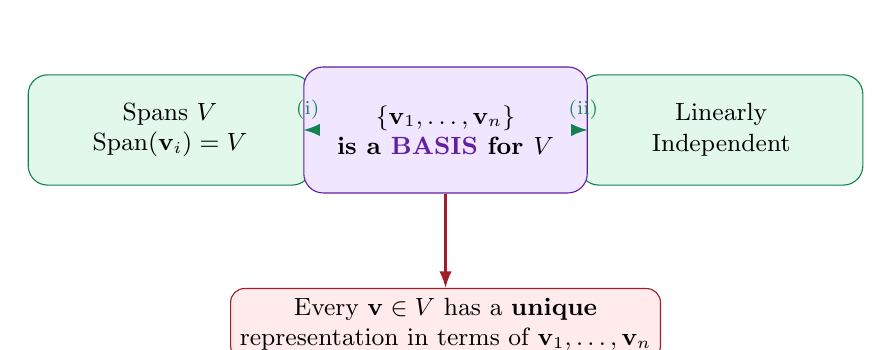
\begin{tikzpicture}[
				mainbox/.style={draw=axiomblue, fill=shadeblue, rounded corners=7pt,
					minimum width=3.6cm, minimum height=1.4cm, align=center,
					font=\small},
				condbox/.style={draw=defgreen, fill=shadegreen, rounded corners=7pt,
					minimum width=3.6cm, minimum height=1.4cm, align=center,
					font=\small},
				basisbox/.style={draw=purpledark, fill=purpleshade, rounded corners=7pt,
					minimum width=3.6cm, minimum height=1.6cm, align=center,
					font=\small\bfseries},
				arr/.style={-{Latex[length=6pt]}, thick}
				]
				\node[condbox] (span) at (-3.5, 0) {Spans $V$\\$\Span(\vv{v}_i) = V$};
				\node[condbox] (ind)  at ( 3.5, 0) {Linearly\\Independent};
				\node[basisbox] (basis) at (0, 0)
				{$\{\vv{v}_1,\ldots,\vv{v}_n\}$\\is a \textcolor{purpledark}{BASIS} for $V$};
				\draw[arr, defgreen] (span) -- (basis)
				node[midway, above, font=\scriptsize]{(i)};
				\draw[arr, defgreen] (ind)  -- (basis)
				node[midway, above, font=\scriptsize]{(ii)};
				\node[draw=thmred, fill=shadered, rounded corners=5pt,
				align=center, font=\small, below=1.2cm of basis] (uniq)
				{Every $\vv{v}\in V$ has a \textbf{unique}\\
					representation in terms of $\vv{v}_1,\ldots,\vv{v}_n$};
				\draw[arr, thmred] (basis) -- (uniq);
			\end{tikzpicture}
		\end{center}
		
		\subsection{Standard Bases}
		
		\begin{example}{Standard basis for $\R^n$}{stdbasisRn}
			The set $\mathcal{E} = \{\vv{e}_1, \vv{e}_2, \ldots, \vv{e}_n\}$, where
			$\vv{e}_i$ is the vector with a $1$ in position $i$ and $0$s elsewhere,
			is the \textbf{standard basis} for $\R^n$:
			\[
			\vv{e}_1 = \begin{pmatrix}1\\0\\\vdots\\0\end{pmatrix},\quad
			\vv{e}_2 = \begin{pmatrix}0\\1\\\vdots\\0\end{pmatrix},\quad
			\ldots,\quad
			\vv{e}_n = \begin{pmatrix}0\\0\\\vdots\\1\end{pmatrix}.
			\]
			For any $\vv{x} = (x_1, \ldots, x_n)^T \in \R^n$:
			$\vv{x} = x_1\vv{e}_1 + \cdots + x_n\vv{e}_n$ (spanning),
			and the only solution to $\sum \alpha_i\vv{e}_i = \vzero$ is
			$\alpha_i = 0$ for all $i$ (independence).
		\end{example}
		
		\begin{example}{Standard basis for $P_n$}{stdbasisPn}
			The set $\{1,\, x,\, x^2,\, \ldots,\, x^{n-1}\}$ is the standard basis for
			$P_n$.  Every $p \in P_n$ writes uniquely as
			$p(x) = a_0 + a_1 x + \cdots + a_{n-1}x^{n-1}$, giving
			coordinates $(a_0, a_1, \ldots, a_{n-1})^T$.
		\end{example}
		
		\begin{example}{Standard basis for $\R^{m \times n}$}{stdbasisMmn}
			For the space $\R^{m\times n}$, define $E_{ij}$ to be the $m\times n$ matrix
			with a $1$ in position $(i,j)$ and $0$s elsewhere.  The set
			$\{E_{ij} : 1 \leq i \leq m,\; 1 \leq j \leq n\}$ is a basis for $\R^{m\times n}$.
			For example, the standard basis of $\R^{2\times 2}$ is:
			\[
			E_{11}=\begin{pmatrix}1&0\\0&0\end{pmatrix},\quad
			E_{12}=\begin{pmatrix}0&1\\0&0\end{pmatrix},\quad
			E_{21}=\begin{pmatrix}0&0\\1&0\end{pmatrix},\quad
			E_{22}=\begin{pmatrix}0&0\\0&1\end{pmatrix}.
			\]
		\end{example}
		
		\subsection{Existence and Reduction of Spanning Sets}
		
		\begin{theorem}{Spanning Set Contains a Basis}{spanbasis}
			Every finite spanning set for a non-zero vector space $V$ contains a basis.
		\end{theorem}
		
		\begin{proof}
			Let $S = \{\vv{v}_1, \ldots, \vv{v}_n\}$ span $V$.  If $S$ is linearly
			independent, it is already a basis.  Otherwise, by
			Theorem~\ref{thm:depspan}, some $\vv{v}_k \in \Span(\vv{v}_1,\ldots,
			\vv{v}_{k-1})$, so removing $\vv{v}_k$ leaves a set that still spans $V$.
			Repeat until the remaining set is linearly independent; the result is a basis.
		\end{proof}
		
		\begin{theorem}{Extending Independent Sets to a Basis}{extbasis}
			Every linearly independent subset of a finite-dimensional vector space $V$
			can be extended to a basis for $V$.
		\end{theorem}
		
		\subsection{Worked Example: Finding a Basis from a Spanning Set}
		
		\begin{example}{Basis for a subspace of $\R^4$}{basisex}
			Find a basis for
			$W = \Span\!\bigl((1,2,1,0)^T,\; (2,4,2,0)^T,\; (1,0,1,2)^T,\;
			(0,2,0,-2)^T\bigr)$.
			
			Place the vectors as rows and row-reduce:
			\[
			\begin{pmatrix}
				1&2&1&0\\ 2&4&2&0\\ 1&0&1&2\\ 0&2&0&-2
			\end{pmatrix}
			\xrightarrow{\substack{R_2-2R_1\\R_3-R_1}}
			\begin{pmatrix}
				1&2&1&0\\ 0&0&0&0\\ 0&-2&0&2\\ 0&2&0&-2
			\end{pmatrix}
			\xrightarrow{R_4+R_3}
			\begin{pmatrix}
				1&2&1&0\\ 0&-2&0&2\\ 0&0&0&0\\ 0&0&0&0
			\end{pmatrix}.
			\]
			The two non-zero rows correspond to the first and third original vectors
			(rows 1 and 3 of the original matrix are the pivot rows).  A basis for
			$W$ is:
			\[
			\bigl\{(1,2,1,0)^T,\; (1,0,1,2)^T\bigr\}.
			\]
		\end{example}
		
		% ══════════════════════════════════════════════════════════════════════════════
		\section{Dimension of a Vector Space}
		\label{sec:dimension}
		% ══════════════════════════════════════════════════════════════════════════════
		
		\subsection{The Dimension Theorem}
		
		\begin{theorem}{All Bases Have the Same Size}{samedim}
			Let $V$ be a vector space.  If $\{\vv{u}_1, \ldots, \vv{m}\}$ and
			$\{\vv{w}_1, \ldots, \vv{w}_n\}$ are both bases for $V$, then $m = n$.
		\end{theorem}
		
		\begin{proof}
			Since $\{\vv{u}_1,\ldots,\vv{u}_m\}$ spans $V$ and
			$\{\vv{w}_1,\ldots,\vv{w}_n\}$ is linearly independent, Theorem~\ref
			{thm:sizebound} gives $n \leq m$.  Symmetrically, $m \leq n$.  Hence $m = n$.
		\end{proof}
		
		\noindent
		This theorem justifies the following definition.
		
		\begin{definition}{Dimension}{dimdef}
			Let $V$ be a vector space.  If $V$ has a basis consisting of exactly $n$
			vectors, we say $V$ is \textbf{finite-dimensional} and define the
			\textbf{dimension} of $V$ to be
			\[
			\dim(V) = n.
			\]
			The zero vector space $\{\vzero\}$ is defined to have dimension $0$.
			If no finite basis exists, $V$ is called \textbf{infinite-dimensional}.
		\end{definition}
		
		\subsection{Dimensions of Common Spaces}
		
		\begin{center}
			\renewcommand{\arraystretch}{1.5}
			\begin{tabular}{>{\bfseries}p{3cm} p{5cm} p{2.5cm} p{2cm}}
				\toprule
				Space & Standard Basis & Dimension & Notes \\
				\midrule
				$\R^n$
				& $\{\vv{e}_1, \ldots, \vv{e}_n\}$
				& $n$
				& \\
				$\R^{m\times n}$
				& $\{E_{ij}\}$, $1\leq i\leq m$, $1\leq j\leq n$
				& $mn$
				& \\
				$P_n$
				& $\{1, x, x^2, \ldots, x^{n-1}\}$
				& $n$
				& \\
				$C[a,b]$
				& No finite basis
				& $\infty$
				& Infinite-dimensional \\
				$\{\vzero\}$
				& Empty set
				& $0$
				& Zero subspace \\
				\bottomrule
			\end{tabular}
		\end{center}
		
		\subsection{Dimension and Subspaces}
		
		\begin{theorem}{Dimension of Subspaces}{dimsub}
			Let $S$ be a subspace of a finite-dimensional vector space $V$.  Then:
			\begin{enumerate}[label=(\roman*), leftmargin=2.5em]
				\item $\dim(S) \leq \dim(V)$.
				\item $\dim(S) = \dim(V)$ if and only if $S = V$.
			\end{enumerate}
		\end{theorem}
		
		\begin{proof}
			\textbf{(i)}\; Any basis of $S$ is a linearly independent set in $V$.
			By Theorem~\ref{thm:sizebound}, its size cannot exceed $\dim(V)$.
			
			\textbf{(ii)}\; If $\dim(S)=\dim(V)=n$, take any basis
			$\{\vv{u}_1,\ldots,\vv{u}_n\}$ of $S$.  Being linearly independent and of
			size $n = \dim(V)$, it is also a basis for $V$ (by Theorem~\ref
			{thm:extbasis}), so $S = \Span(\vv{u}_1,\ldots,\vv{u}_n) = V$.
		\end{proof}
		
		\noindent
		The diagram below shows how dimension stratifies the subspaces of $\R^3$:
		
		\begin{center}
			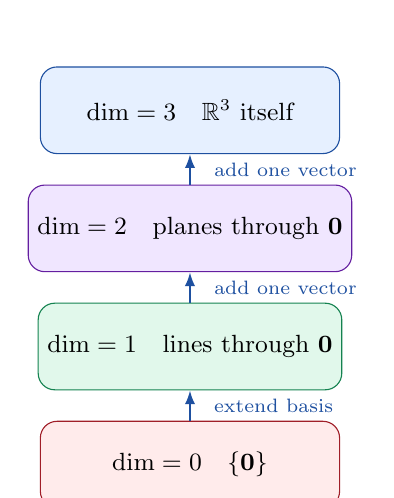
\begin{tikzpicture}[
				dimbox/.style={draw=axiomblue, fill=shadeblue, rounded corners=6pt,
					minimum width=3.8cm, minimum height=1.1cm,
					align=center, font=\small},
				arr/.style={-{Latex[length=5pt]}, axiomblue, thick}
				]
				\node[dimbox] (d3) at (0, 4.5)
				{$\dim = 3$\quad $\R^3$ itself};
				\node[dimbox, fill=purpleshade, draw=purpledark] (d2) at (0, 3.0)
				{$\dim = 2$\quad planes through $\vzero$};
				\node[dimbox, fill=shadegreen, draw=defgreen] (d1) at (0, 1.5)
				{$\dim = 1$\quad lines through $\vzero$};
				\node[dimbox, fill=shadered, draw=thmred] (d0) at (0, 0)
				{$\dim = 0$\quad $\{\vzero\}$};
				\draw[arr] (d0) -- (d1) node[midway, right=5pt, font=\scriptsize]{extend basis};
				\draw[arr] (d1) -- (d2) node[midway, right=5pt, font=\scriptsize]{add one vector};
				\draw[arr] (d2) -- (d3) node[midway, right=5pt, font=\scriptsize]{add one vector};
			\end{tikzpicture}
		\end{center}
		
		\subsection{A Practical Characterisation}
		
		\begin{theorem}{Three Equivalent Conditions}{equiv3}
			Let $V$ be an $n$-dimensional vector space and let
			$S = \{\vv{v}_1, \ldots, \vv{v}_n\}$ be any set of exactly $n$ vectors in $V$.
			Then the following are equivalent:
			\begin{enumerate}[label=(\roman*), leftmargin=2.5em]
				\item $S$ is a basis for $V$.
				\item $S$ spans $V$.
				\item $S$ is linearly independent.
			\end{enumerate}
		\end{theorem}
		
		\begin{proof}
			\textbf{(i)$\Rightarrow$(ii) and (i)$\Rightarrow$(iii)} follow directly from
			the definition of basis.
			
			\textbf{(ii)$\Rightarrow$(i)}\; If $S$ spans $V$, it contains a basis
			(Theorem~\ref{thm:spanbasis}).  That basis has $n = \dim(V)$ vectors, and
			since $|S| = n$, removing any vector would make $|S| < n$, so $S$ itself is
			the basis.
			
			\textbf{(iii)$\Rightarrow$(i)}\; If $S$ is linearly independent, extend it
			to a basis $B$ (Theorem~\ref{thm:extbasis}); since $|B| = n = |S|$, we have
			$B = S$, so $S$ is a basis.
		\end{proof}
		
		% ══════════════════════════════════════════════════════════════════════════════
		\section{Rank, Nullity, and the Rank--Nullity Theorem}
		\label{sec:ranknullity}
		% ══════════════════════════════════════════════════════════════════════════════
		
		\subsection{Row Space, Column Space, and Rank}
		
		\begin{definition}{Row Space and Column Space}{rowcol}
			Let $A$ be an $m \times n$ matrix.
			\begin{itemize}[leftmargin=2em]
				\item The \textbf{row space} of $A$, denoted $\text{Row}(A)$, is the span
				of the row vectors of $A$, viewed as a subspace of $\R^n$.
				\item The \textbf{column space} of $A$, denoted $\text{Col}(A)$, is the
				span of the column vectors of $A$, viewed as a subspace of $\R^m$.
				\item The \textbf{rank} of $A$ is
				$\rank(A) = \dim(\text{Row}(A)) = \dim(\text{Col}(A))$.
				\item The \textbf{nullity} of $A$ is
				$\nullity(A) = \dim(N(A))$.
			\end{itemize}
		\end{definition}
		
		\subsection{The Rank--Nullity Theorem}
		
		\begin{theorem}{Rank--Nullity Theorem}{ranknull}
			For any $m \times n$ matrix $A$,
			\[
			\rank(A) + \nullity(A) = n.
			\]
		\end{theorem}
		
		\begin{proof}
			Let $r = \rank(A)$.  Row-reduction of $A$ produces $r$ pivot columns and
			$n - r$ free columns.  The $n - r$ free variables parametrise $N(A)$; the
			corresponding $n - r$ special solutions form a basis for $N(A)$, so
			$\nullity(A) = n - r$.  Therefore $r + (n-r) = n$.
		\end{proof}
		
		\noindent
		The Rank--Nullity Theorem can be visualised as a partition of $\R^n$:
		
		\begin{center}
			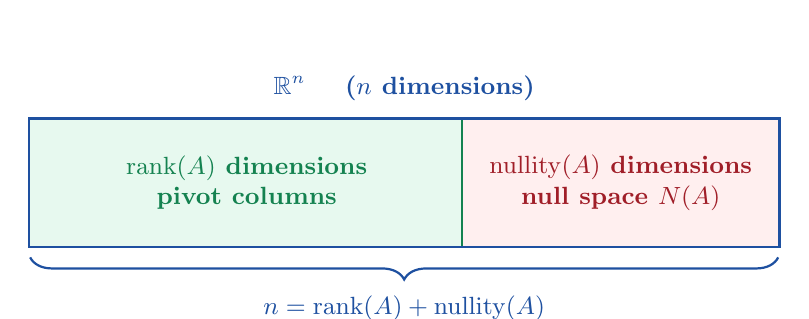
\begin{tikzpicture}[scale=1.0]
				% Full rectangle = R^n (n columns)
				\draw[axiomblue, line width=1.8pt]
				(0,0) rectangle (9.5, 1.6);
				\node[axiomblue, font=\small\bfseries] at (4.75, 2.0)
				{$\R^n$ \quad ($n$ dimensions)};
				% Left part = rank(A) = column space pre-image
				\fill[shadegreen!80] (0,0) rectangle (5.5, 1.6);
				\draw[defgreen, line width=1.4pt] (5.5, 0) -- (5.5, 1.6);
				\node[defgreen, font=\small\bfseries, align=center] at (2.75, 0.8)
				{$\rank(A)$ dimensions\\pivot columns};
				% Right part = nullity(A) = null space
				\fill[shadered!80] (5.5,0) rectangle (9.5,1.6);
				\node[thmred, font=\small\bfseries, align=center] at (7.5, 0.8)
				{$\nullity(A)$ dimensions\\null space $N(A)$};
				% brace below
				\draw[decorate,
				decoration={brace, amplitude=8pt, mirror},
				axiomblue, thick]
				(0,-0.15) -- (9.5,-0.15)
				node[midway, below=10pt, font=\small, axiomblue]
				{$n = \rank(A) + \nullity(A)$};
			\end{tikzpicture}
		\end{center}
		
		\subsection{Worked Example}
		
		\begin{example}{Rank, nullity and the theorem}{rnex}
			Let
			\[
			A = \begin{pmatrix}
				1 & 2 & 0 & 1 \\
				2 & 4 & 1 & 3 \\
				0 & 0 & 1 & 1
			\end{pmatrix}.
			\]
			Row-reduce:
			\[
			\begin{pmatrix}
				1&2&0&1\\2&4&1&3\\0&0&1&1
			\end{pmatrix}
			\xrightarrow{R_2 - 2R_1}
			\begin{pmatrix}
				1&2&0&1\\0&0&1&1\\0&0&1&1
			\end{pmatrix}
			\xrightarrow{R_3 - R_2}
			\begin{pmatrix}
				1&2&0&1\\0&0&1&1\\0&0&0&0
			\end{pmatrix}.
			\]
			There are $2$ pivot columns (columns 1 and 3), so $\rank(A) = 2$.
			The free variables are $x_2$ and $x_4$, so $\nullity(A) = 2$.
			Indeed: $\rank(A) + \nullity(A) = 2 + 2 = 4 = n$. \checkmark
			
			A basis for $N(A)$ (setting $(x_2,x_4) = (1,0)$ then $(0,1)$):
			\[
			N(A) = \Span\!\left(
			\begin{pmatrix}-2\\1\\0\\0\end{pmatrix},\;
			\begin{pmatrix}-1\\0\\-1\\1\end{pmatrix}
			\right).
			\]
		\end{example}
		
		% ══════════════════════════════════════════════════════════════════════════════
		\section{Summary and Connections}
		% ══════════════════════════════════════════════════════════════════════════════
		
		\begin{tcolorbox}[
			enhanced, colback=shadeyellow, colframe=orange!70!black,
			title={\bfseries Chapter Summary}, breakable
			]
			\begin{itemize}[leftmargin=1.5em, itemsep=0.5em]
				\item Vectors $\vv{v}_1, \ldots, \vv{v}_n$ are \textbf{linearly independent}
				iff $\sum\alpha_i\vv{v}_i = \vzero \Rightarrow$ all $\alpha_i = 0$.
				Otherwise they are \textbf{linearly dependent} and some vector is
				redundant.
				\item A \textbf{basis} for $V$ is a linearly independent spanning set.
				Every vector in $V$ has a \emph{unique} coordinate representation in
				any basis.
				\item All bases of a finite-dimensional vector space $V$ have the same
				number of elements; this common count is $\dim(V)$.
				\item Any $\dim(V)$ vectors that span $V$, or that are linearly
				independent, automatically form a basis.
				\item For an $m\times n$ matrix $A$: $\rank(A) + \nullity(A) = n$
				(Rank--Nullity Theorem).
			\end{itemize}
		\end{tcolorbox}
		
		\medskip
		\noindent
		The diagram below summarises the relationships among all key concepts.
		
		\begin{center}
			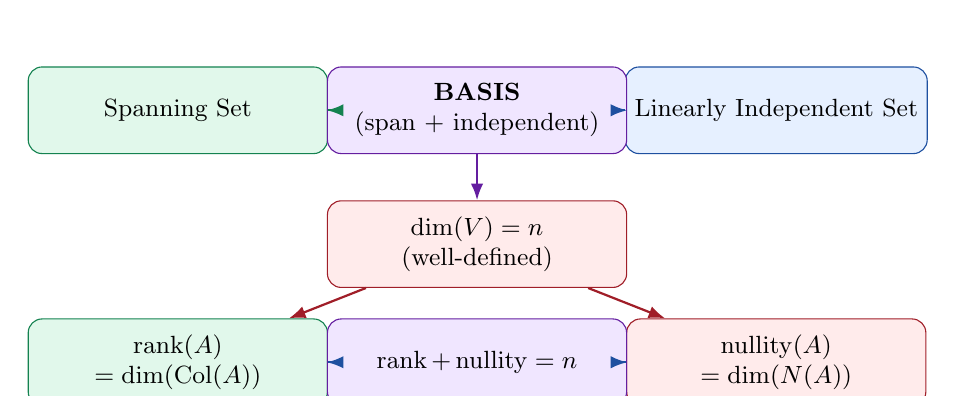
\begin{tikzpicture}[
				cbox/.style={draw=axiomblue, fill=shadeblue, rounded corners=5pt,
					minimum width=3.8cm, minimum height=1.1cm,
					align=center, font=\small},
				gbox/.style={draw=defgreen, fill=shadegreen, rounded corners=5pt,
					minimum width=3.8cm, minimum height=1.1cm,
					align=center, font=\small},
				rbox/.style={draw=thmred, fill=shadered, rounded corners=5pt,
					minimum width=3.8cm, minimum height=1.1cm,
					align=center, font=\small},
				pbox/.style={draw=purpledark, fill=purpleshade, rounded corners=5pt,
					minimum width=3.8cm, minimum height=1.1cm,
					align=center, font=\small},
				arr/.style={-{Latex[length=6pt]}, thick}
				]
				\node[gbox] (span) at (-3.8, 2.2)  {Spanning Set};
				\node[cbox] (ind)  at ( 3.8, 2.2)  {Linearly Independent Set};
				\node[pbox] (basis) at (0,   2.2)  {\textbf{BASIS}\\(span $+$ independent)};
				\node[rbox] (dim)  at (0,   0.5)   {$\dim(V) = n$\\(well-defined)};
				\node[gbox] (rank) at (-3.8,-1.0)  {$\rank(A)$\\$= \dim(\text{Col}(A))$};
				\node[rbox] (null) at ( 3.8,-1.0)  {$\nullity(A)$\\$= \dim(N(A))$};
				\node[pbox] (rnt)  at (0,  -1.0)   {$\rank + \nullity = n$};
				\draw[arr, defgreen]  (span)  -- (basis);
				\draw[arr, axiomblue] (ind)   -- (basis);
				\draw[arr, purpledark](basis) -- (dim);
				\draw[arr, thmred]    (dim)   -- (rank);
				\draw[arr, thmred]    (dim)   -- (null);
				\draw[arr, axiomblue] (rank)  -- (rnt);
				\draw[arr, axiomblue] (null)  -- (rnt);
			\end{tikzpicture}
		\end{center}
		
		% ══════════════════════════════════════════════════════════════════════════════
	\end{document}
	% ══════════════════════════════════════════════════════════════════════════════